\input{Dissertation/appendixsetup}   % Предварительные настройки для правильного подключения Приложений
\chapter{Визуализация примера <<Hello World!>>} \label{AppendixA}

\begin{figure*}[h]
	\centering
	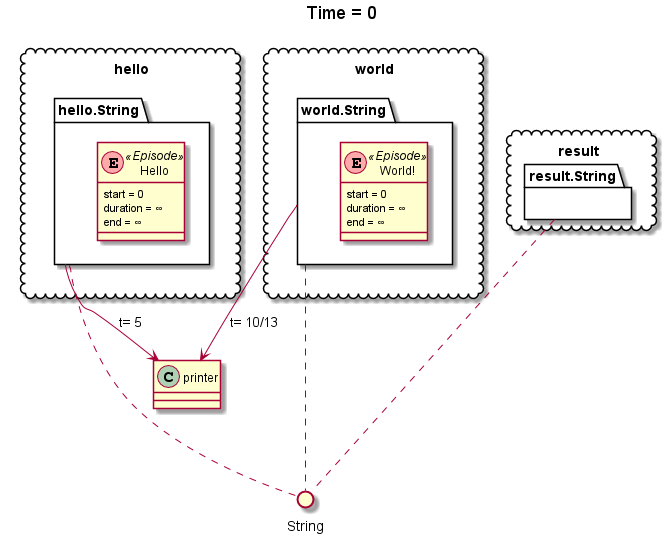
\includegraphics[width=0.7\linewidth]{state0}
	\caption{Визуализация примера из листинга \ref{list:interface}. Состояние 1.}
	\label{fig:state1}
\end{figure*}

\begin{figure*}[h]
	\centering
	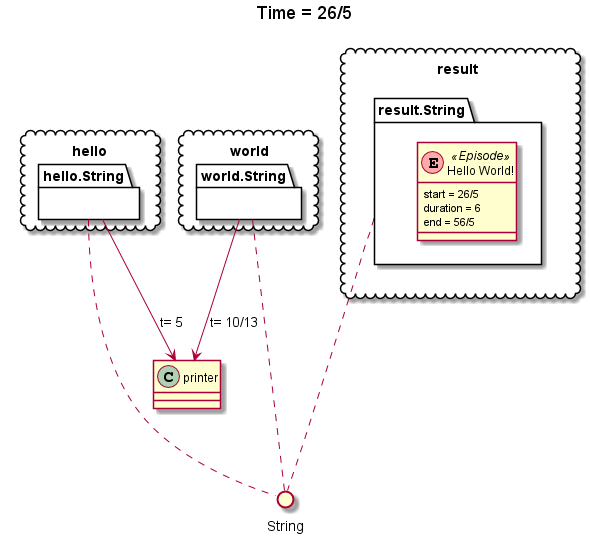
\includegraphics[width=0.7\linewidth]{state1}
	\caption{Визуализация примера из листинга \ref{list:interface}. Состояние 2.}
	\label{fig:state2}
\end{figure*}


%\section{Пример работы}
\begin{figure*}[h]
	\centering
	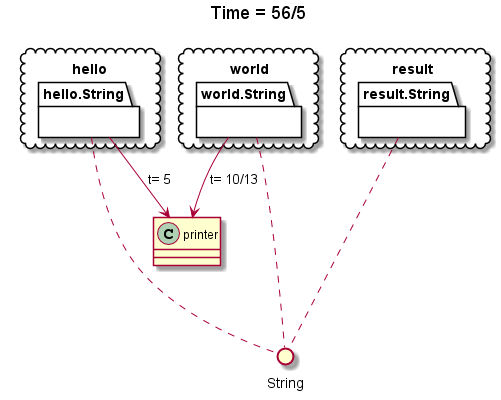
\includegraphics[width=0.7\linewidth]{state2}
	\caption{Визуализация примера из листинга \ref{list:interface}. Состояние 3.}
	\label{fig:state3}
\end{figure*}

\chapter{Пример нахождения НОД алгоритмом Евклида} \label{AppendixB}

\lstinputlisting[lastline=264, language={Kotlin}, caption={Реализация алгоритма Евклида на языке динамических систем.}, label={list:euclidean}] {listings/euclidean.kt}

\begin{figure*}[h]
	\centering
	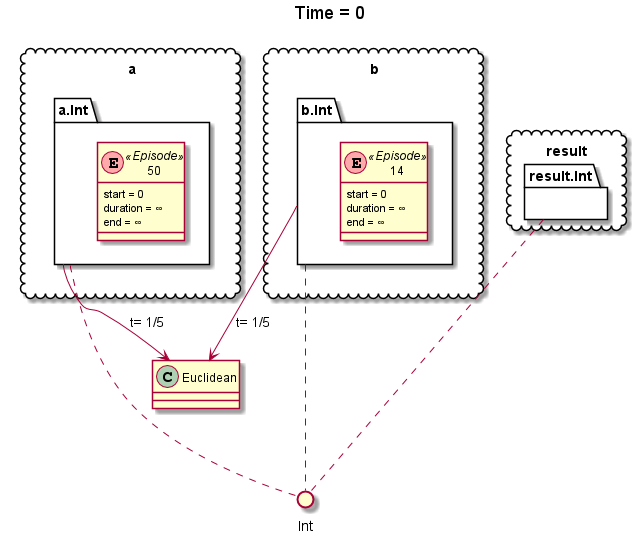
\includegraphics[width=0.7\linewidth]{images/euclidean1}
	\caption{НОД(50,14). Состояние 1.}
	\label{fig:euclidean1}
\end{figure*}
\begin{figure*}[h]
	\centering
	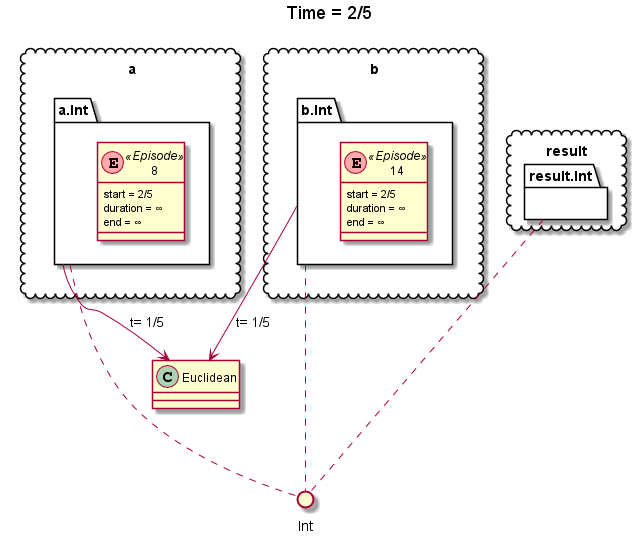
\includegraphics[width=0.7\linewidth]{images/euclidean2}
	\caption{НОД(50,14). Состояние 2.}
	\label{fig:euclidean2}
\end{figure*}
\begin{figure*}[h]
	\centering
	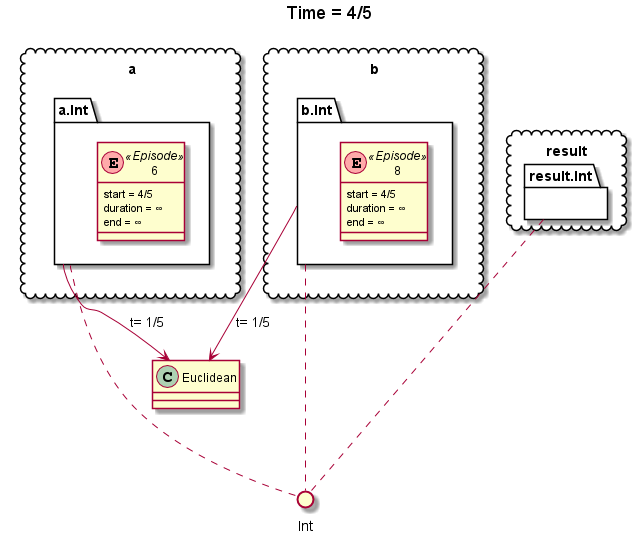
\includegraphics[width=0.7\linewidth]{images/euclidean3}
	\caption{НОД(50,14). Состояние 3.}
	\label{fig:euclidean3}
\end{figure*}
\begin{figure*}[h]
	\centering
	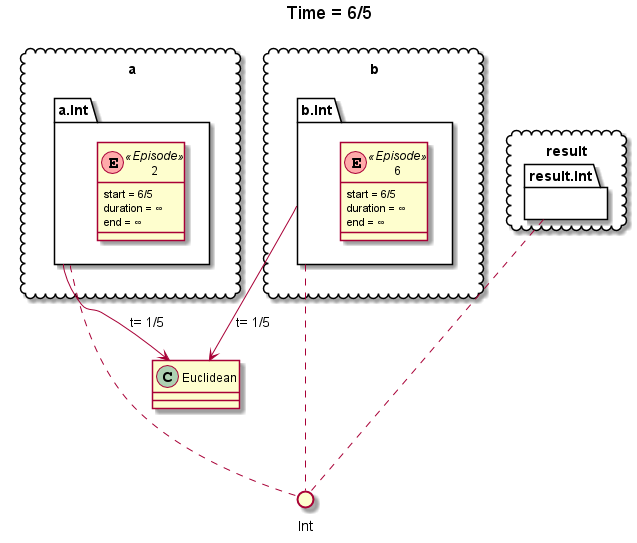
\includegraphics[width=0.7\linewidth]{images/euclidean4}
	\caption{НОД(50,14). Состояние 4.}
	\label{fig:euclidean4}
\end{figure*}
\begin{figure*}[h]
	\centering
	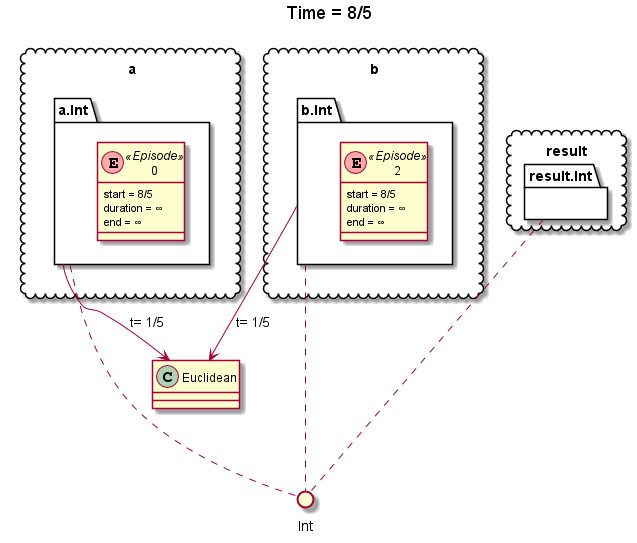
\includegraphics[width=0.7\linewidth]{images/euclidean5}
	\caption{НОД(50,14). Состояние 5.}
	\label{fig:euclidean5}
\end{figure*}
\begin{figure*}[h]
	\centering
	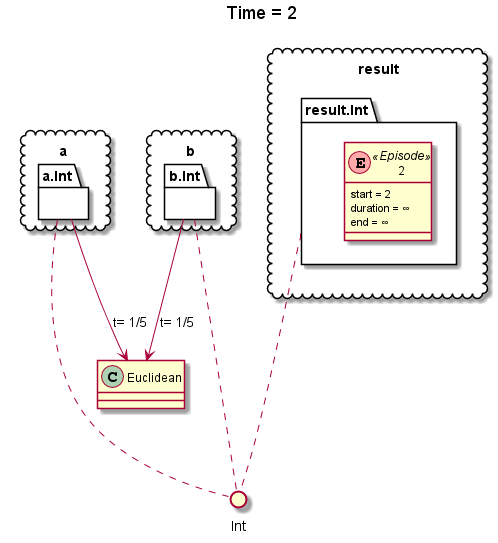
\includegraphics[width=0.5\linewidth]{images/euclidean6}
	\caption{НОД(50,14). Состояние 6. Результат.}
	\label{fig:euclidean6}
\end{figure*}



\chapter{Исходный код программы}
\lstinputlisting[lastline=264, language={Kotlin}, caption={DataModel.kt}, label={list:datamodel}] {listings/DataModel.kt}

\lstinputlisting[lastline=66, language={Kotlin}, caption={DSL}, label={list:dsl}] {listings/DSL.kt}


\lstinputlisting[lastline=96, language={Kotlin}, caption={Time.kt}, label={list:time}] {listings/Time.kt}

\lstinputlisting[lastline=129, language={Kotlin}, caption={Process.kt}, label={list:process}] {listings/Process.kt}

\lstinputlisting[lastline=62, language={Kotlin}, caption={PlantUML.kt}, label={list:plantuml}] {listings/PlantUML.kt}